\chapter{Funcionamiento del programa}

\color{blue}

El propósito principal del programa \textit{molmassfractaldim} es determinar la dimesi\'{o}n fractal de masa mediante la caracterizaci\'{o}n de la geometría interna de un sistema proteico. Esto se logra construyendo una tabla de $r_{k}$, $\langle N(r_k) \rangle$, $\langle M(r_k) \rangle$ y $\langle Rg(r_k) \rangle$: donde;

\begin{itemize}
	\item $r_{k}$ es el radio de medida centrado en posiciones aleatorias de una prote\'{i}na con valores m\'{i}nimos y m\'{a}ximos definidos como $r_{min}$ y $r_{max}$.
	\item $\langle N(r_k) \rangle$ es el número promedio de partículas contenidas dentro de un radio $r_{k}$. 
	\item  $\langle M(r_k) \rangle$ es el n\'{u}mero de masa promedio de las part\'{i}culas contenidas en el radio $r_{k}$.
	\item  $\langle Rg(r_k) \rangle$ es el radio de giro promedio de las part\'{i}culas contenidas en el radio $r_{k}$.
\end{itemize}

Posteriormente, los valores de $\langle N(r_k) \rangle$, $\langle M(r_k) \rangle$ y $\langle Rg(r_k) \rangle$ pueden analizarse mediante regresiones lineales para determinar la dimensi\'{o}n fractal de masa.


	\clearpage

\subsection*{Banderas de entrada}

	El programa \emph{molmassfractaldim}, incorpora banderas de entrada al c\'{o}digo para tener distintas opciones en el c\'{a}lculo de la dimensi\'{o}n fractal de masa. Las banderas incorporadas se muestran en la Tabla \ref{tab:opciones_programa}.
	
	\begin{table}[H]
		\centering
		\begin{tabular}{lp{11cm}}
			\hline
			\textbf{Opci\'{o}n} & \textbf{Descripci\'{o}n} \\ \hline
			-a A & Establece el n\'{u}mero de medidas a realizar. Esto se refiere a la cantidad de veces que el programa calcular\'{a} el promedio de $\langle N(r_k) \rangle$ $\langle M(r_k) \rangle$ y $\langle R_g(r_k) \rangle$. Es \'{u}til si se desea promediar los resultados sobre diferentes configuraciones o pruebas. Para más detalles sobre esta opción, véase la sección \ref{sec:detM(r)}. 
			\\ 
			-n k & Define el n\'{u}mero de radios $r_{k}$ que se utilizar\'{a}n. Es decir, el n\'{u}mero de filas en la tabla de $r_{k}$, $\langle N(r_k) \rangle$, $\langle M(r_k) \rangle$ y $\langle Rg(r_k) \rangle$.
			\\
			-l & Permite espaciar los radios multiplicativamente. Es decir, los radios de medición están igualmente separados en una escala logarítmica, en lugar de una escala lineal.
			\\
			-q & Modo silencioso. Al activar esta opci\'{o}n, la mayor\'{i}a de los mensajes informativos que normalmente se mostrar\'{i}an en la salida est\'{a}ndar se suprimir\'{a}n. 
			\\ 
			-r rmn & Establece el radio m\'{i}nimo $r_{min}$ para las mediciones. Esto es \'{u}til para limitar el rango de los radios de las esferas que se tomar\'{a}n en cuenta en los c\'{a}lculos; $r$ se refiere al radio de la esfera. \\ 
			-R rmx & Establece el radio m\'{a}ximo $r_{max}$ para las mediciones. Similar a la opci\'{o}n anterior, permite definir el rango m\'{a}ximo de los radios de las esferas. 
			\\ 
			-V & Muestra la versi\'{o}n del programa. 
			\\ 
			-h & Muestra el men\'{u} de ayuda con la descripci\'{o}n de las opciones y el uso del programa. 
			\\ \hline
		\end{tabular}
		\caption{Banderas de entrada para el programa \emph{molmassfractaldim}.}
		\label{tab:opciones_programa}
	\end{table}
\color{black}

\chapter{Conjunto de 9 proteínas}

	\begin{figure}[H]
	\subsection*{IdPDB:1a2b}	
	\hspace{-0.3cm} 
	\begin{subfigure}{0.49\textwidth}
		\centering
		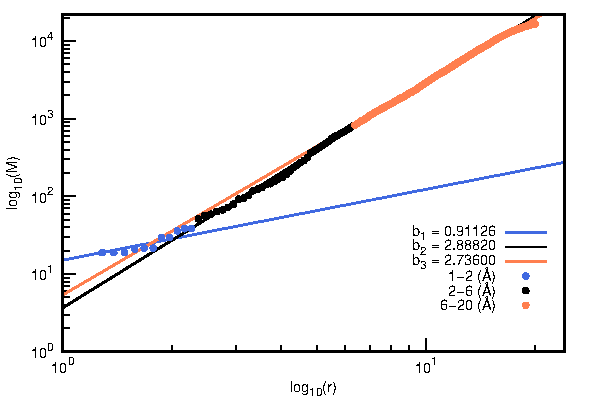
\includegraphics[width=\linewidth,page=1]{graphs/PDBs/1a2b/1a2baddH.pdf}
		\caption{(1)}
	\end{subfigure}
	\hspace{0.2cm}
	\begin{subfigure}{0.49\textwidth}
		\centering
		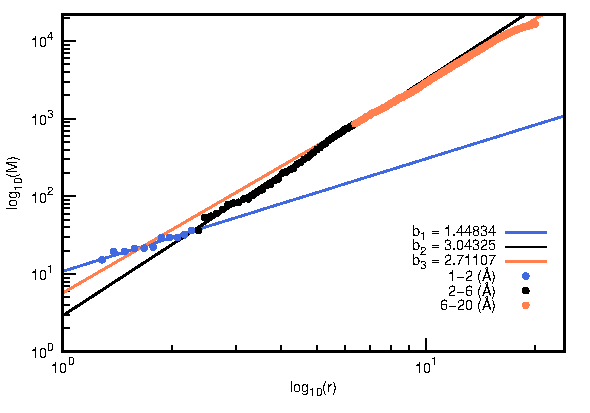
\includegraphics[width=\linewidth,page=1]{graphs/PDBs/1a2b/1a2bEm.pdf}
		\caption{(2)}
	\end{subfigure}
	
	\vspace{0cm} % Espacio entre filas
	
	\hspace{-0.3cm} 
	\begin{subfigure}{0.49\textwidth}
		\centering
		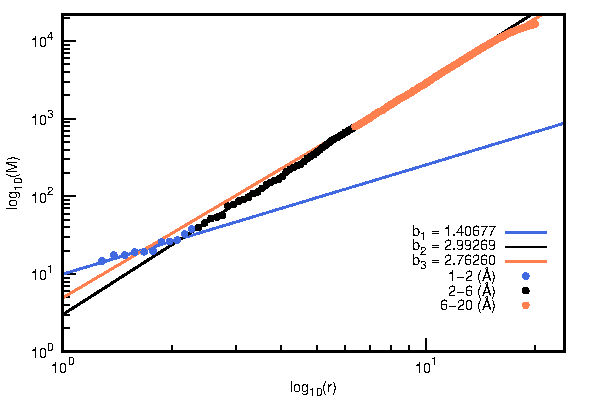
\includegraphics[width=\linewidth,page=1]{graphs/PDBs/1a2b/1a2bEq.pdf}
		\caption{(3)}
	\end{subfigure}
	\hspace{0.2cm}
	\begin{subfigure}{0.49\textwidth} % M\'{a}s ancho para centrar
		\centering
		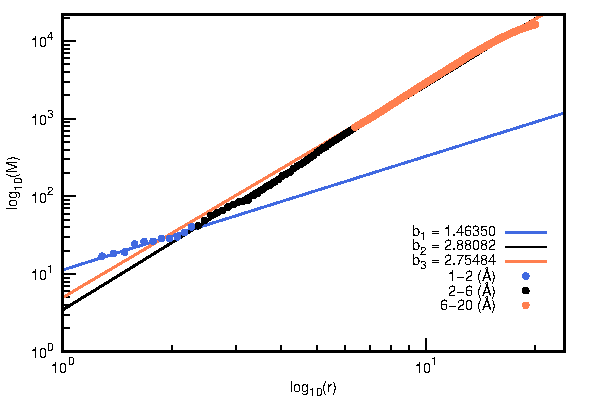
\includegraphics[width=\linewidth,page=1]{graphs/PDBs/1a2b/1a2b1ns.pdf}
		\caption{(4)}
	\end{subfigure}
	
	\caption{
		Regresiones lineales de $\log_{10}r$ vs $\log_{10}M(r)$ correspondiente a cuatro etapas de procesamiento de la primera prote\'{i}na con \textit{IdPDB:1a2b} de la Tabla \ref{Tabla:ids9}: (1) Adici\'{o}n de \'{a}tomos de hidr\'{o}geno al sistema proteico; (2) al minimizar la energ\'{i´}a de la estructura molecular; (3) equilibrando el sistema bajo condiciones termodin\'{a}micas controladas; y (4) despu\'{e}s de una din\'{a}mica molecular de 1 ns.}
	\label{fig:1a2b}
\end{figure}

\begin{figure}[H]
	\subsection*{IdPDB:1a3n}
	
	\hspace{-0.3cm} 
	\begin{subfigure}{0.49\textwidth}
		\centering
		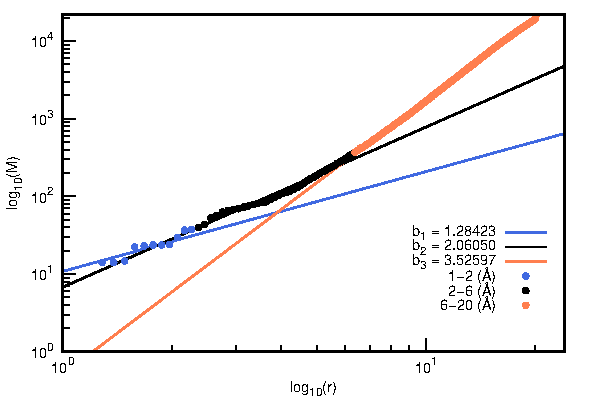
\includegraphics[width=\linewidth,page=1]{graphs/PDBs/1a3n/1a3naddH.pdf}
		\caption{(1)}
	\end{subfigure}
	\hspace{0.2cm}
	\begin{subfigure}{0.49\textwidth}
		\centering
		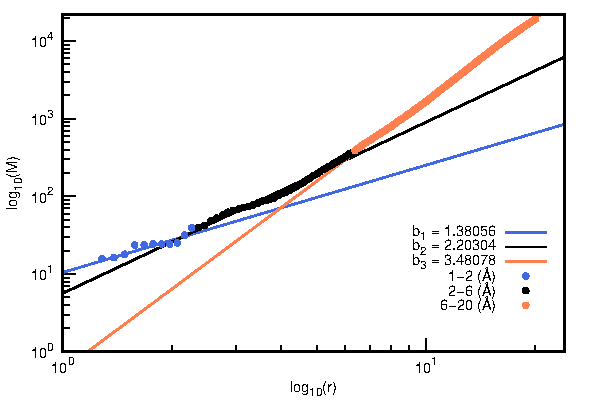
\includegraphics[width=\linewidth,page=1]{graphs/PDBs/1a3n/1a3nEm.pdf}
		\caption{(2)}
	\end{subfigure}
	
	\vspace{0cm} % Espacio entre filas
	
	\hspace{-0.3cm} 
	\begin{subfigure}{0.49\textwidth}
		\centering
		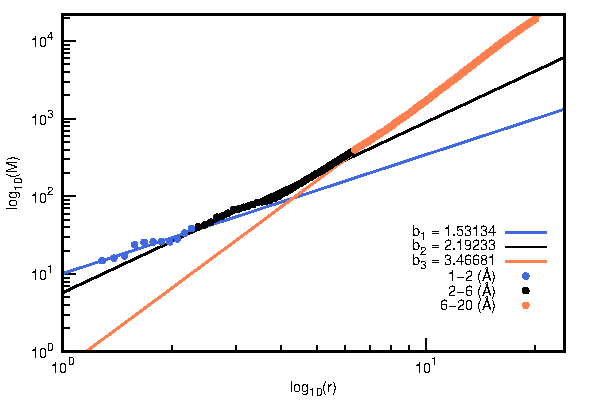
\includegraphics[width=\linewidth,page=1]{graphs/PDBs/1a3n/1a3nEq.pdf}
		\caption{(3)}
	\end{subfigure}
	\hspace{0.2cm}
	\begin{subfigure}{0.49\textwidth} % M\'{a}s ancho para centrar
		\centering
		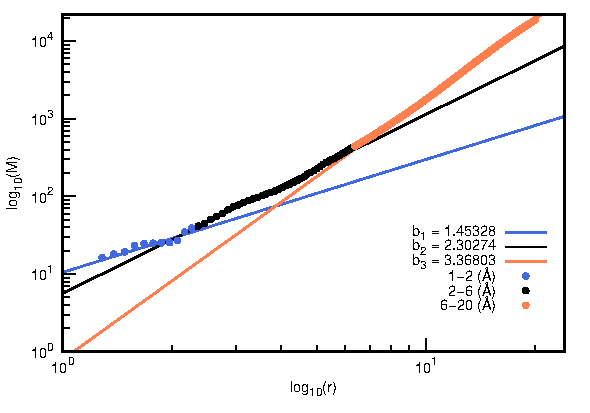
\includegraphics[width=\linewidth,page=1]{graphs/PDBs/1a3n/1a3n1ns.pdf}
		\caption{(4)}
	\end{subfigure}
	\caption{Regresiones lineales de $\log_{10}r$ vs $\log_{10}M(r)$ correspondiente a cuatro etapas de procesamiento de la segunda prote\'{i}na con \textit{IdPDB:1a3n} de la Tabla \ref{Tabla:ids9}: (1) Adici\'{o}n de \'{a}tomos de hidr\'{o}geno al sistema proteico; (2) al minimizar la energ\'{i´}a de la estructura molecular; (3) equilibrando el sistema bajo condiciones termodin\'{a}micas controladas; y (4) despu\'{e}s de una din\'{a}mica molecular de 1 ns.}
	\label{fig:1a3n}
\end{figure}

\begin{figure}[H]
	\subsection*{IdPDB:1a8m}
	
	\hspace{-0.3cm} 
	\begin{subfigure}{0.49\textwidth}
		\centering
		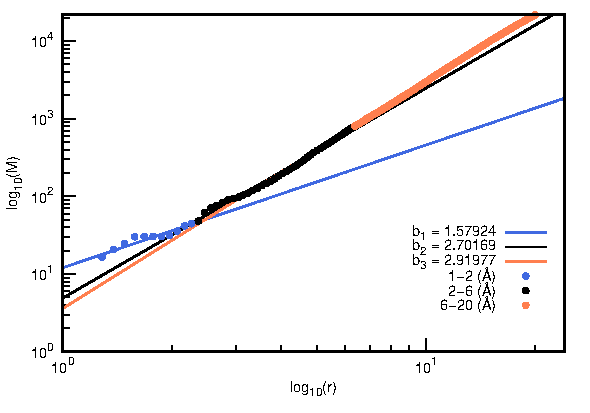
\includegraphics[width=\linewidth,page=1]{graphs/PDBs/1a8m/1a8maddH.pdf}
		\caption{(1)}
	\end{subfigure}
	\hspace{0.2cm}
	\begin{subfigure}{0.49\textwidth}
		\centering
		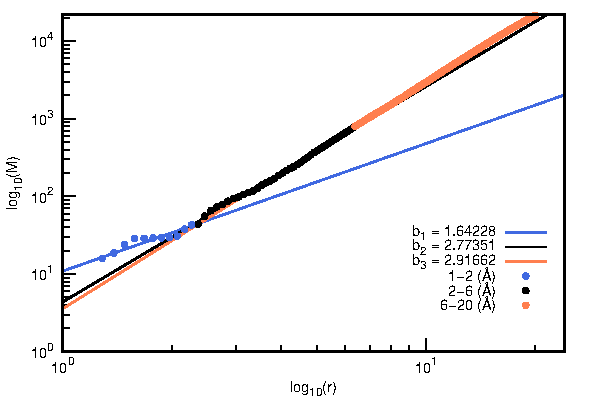
\includegraphics[width=\linewidth,page=1]{graphs/PDBs/1a8m/1a8mEm.pdf}
		\caption{(2)}
	\end{subfigure}
	
	\vspace{0cm} % Espacio entre filas
	
	\hspace{-0.3cm} 
	\begin{subfigure}{0.49\textwidth}
		\centering
		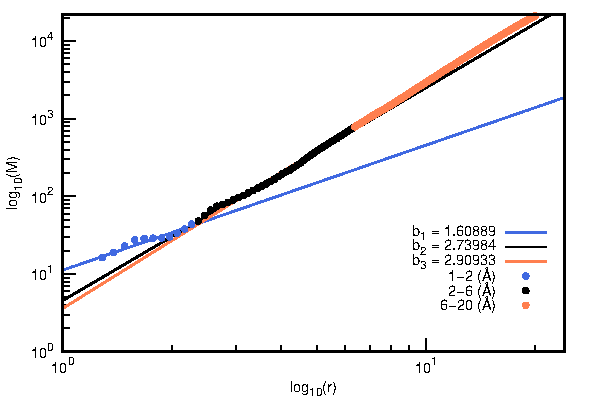
\includegraphics[width=\linewidth,page=1]{graphs/PDBs/1a8m/1a8mEq.pdf}
		\caption{(3)}
	\end{subfigure}
	\hspace{0.2cm}
	\begin{subfigure}{0.49\textwidth} % M\'{a}s ancho para centrar
		\centering
		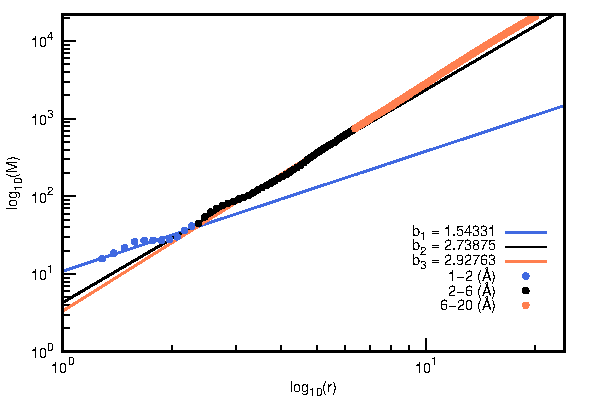
\includegraphics[width=\linewidth,page=1]{graphs/PDBs/1a8m/1a8m1ns.pdf}
		\caption{(4)}
	\end{subfigure}
	\caption{Regresiones lineales de $\log_{10}r$ vs $\log_{10}M(r)$ correspondiente a cuatro etapas de procesamiento de la cuarta prote\'{i}na con \textit{IdPDB:1a8m} de la Tabla \ref{Tabla:ids9}: (1) Adici\'{o}n de \'{a}tomos de hidr\'{o}geno al sistema proteico; (2) al minimizar la energ\'{i´}a de la estructura molecular; (3) equilibrando el sistema bajo condiciones termodin\'{a}micas controladas; y (4) despu\'{e}s de una din\'{a}mica molecular de 1 ns.}
	\label{fig:1a8m}
\end{figure}


\begin{figure}[H]
	\subsection*{IdPDB:1a9w}
	
	\hspace{-0.3cm} 
	\begin{subfigure}{0.49\textwidth}
		\centering
		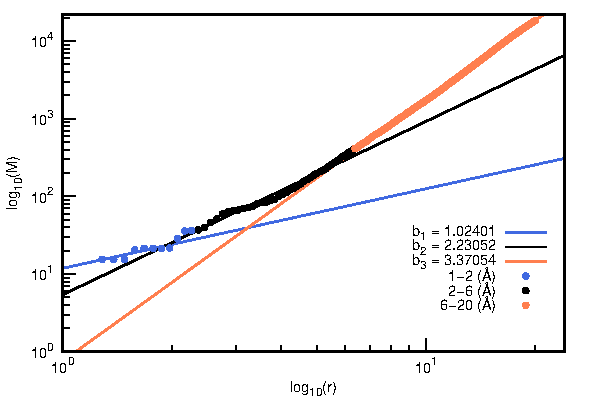
\includegraphics[width=\linewidth,page=1]{graphs/PDBs/1a9w/1a9waddH.pdf}
		\caption{(1)}
	\end{subfigure}
	\hspace{0.2cm}
	\begin{subfigure}{0.49\textwidth}
		\centering
		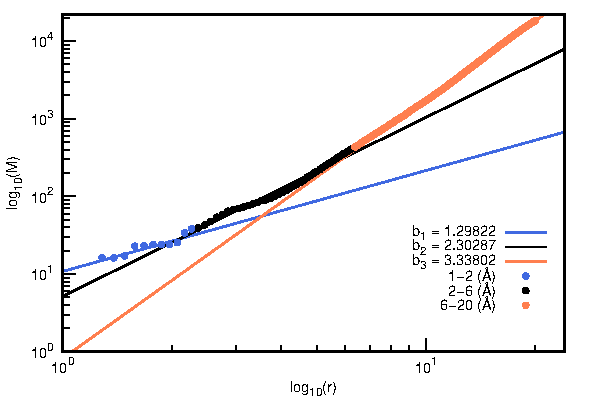
\includegraphics[width=\linewidth,page=1]{graphs/PDBs/1a9w/1a9wEm.pdf}
		\caption{(2)}
	\end{subfigure}
	
	\vspace{0cm} % Espacio entre filas
	
	\hspace{-0.3cm} 
	\begin{subfigure}{0.49\textwidth}
		\centering
		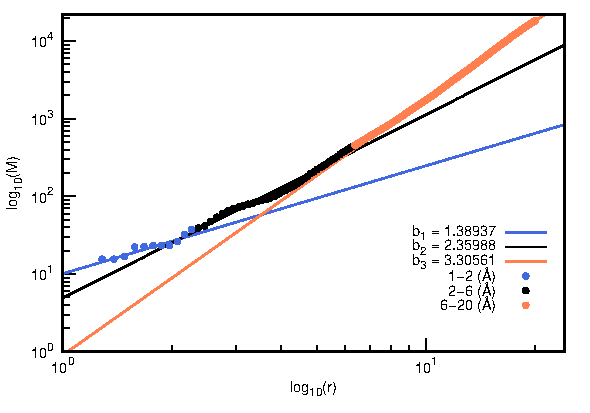
\includegraphics[width=\linewidth,page=1]{graphs/PDBs/1a9w/1a9wEq.pdf}
		\caption{(3)}
	\end{subfigure}
	\hspace{0.2cm}
	\begin{subfigure}{0.49\textwidth} % M\'{a}s ancho para centrar
		\centering
		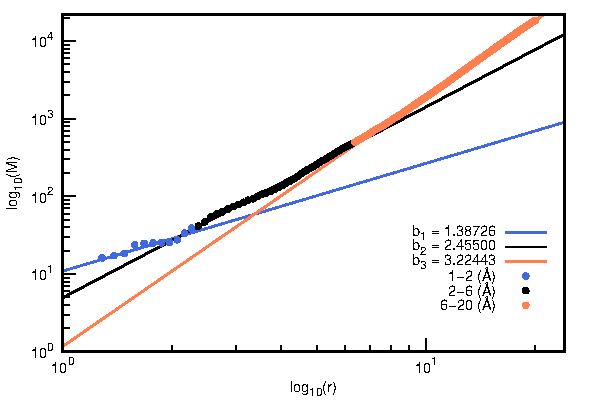
\includegraphics[width=\linewidth,page=1]{graphs/PDBs/1a9w/1a9w1ns.pdf}
		\caption{(4)}
	\end{subfigure}
	\caption{Regresiones lineales de $\log_{10}r$ vs $\log_{10}M(r)$ correspondiente a cuatro etapas de procesamiento de la quinta prote\'{i}na con \textit{IdPDB:1a9w} de la Tabla \ref{Tabla:ids9}: (1) Adici\'{o}n de \'{a}tomos de hidr\'{o}geno al sistema proteico; (2) al minimizar la energ\'{i´}a de la estructura molecular; (3) equilibrando el sistema bajo condiciones termodin\'{a}micas controladas; y (4) despu\'{e}s de una din\'{a}mica molecular de 1 ns.}
	\label{fig:1a9w}
\end{figure}

\begin{figure}[H]
	\subsection*{IdPDB:1a52}
	
	\hspace{-0.3cm} 
	\begin{subfigure}{0.49\textwidth}
		\centering
		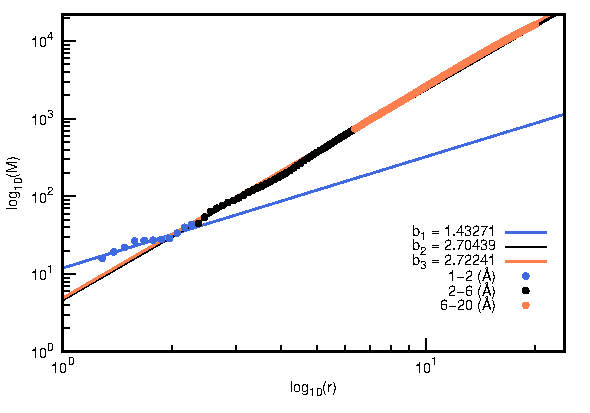
\includegraphics[width=\linewidth,page=1]{graphs/PDBs/1a52/1a52addH.pdf}
		\caption{(1)}
	\end{subfigure}
	\hspace{0.2cm}
	\begin{subfigure}{0.49\textwidth}
		\centering
		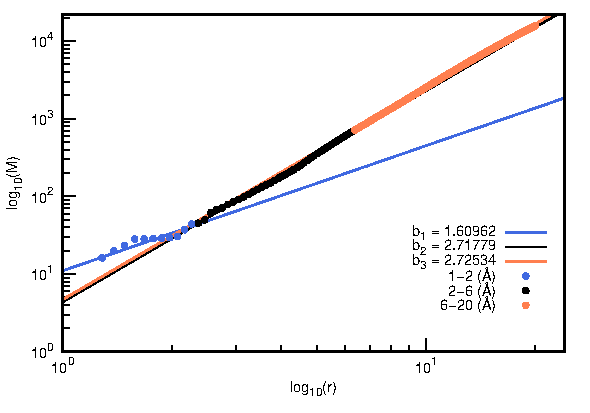
\includegraphics[width=\linewidth,page=1]{graphs/PDBs/1a52/1a52Em.pdf}
		\caption{(2)}
	\end{subfigure}
	
	\vspace{0cm} % Espacio entre filas
	
	\hspace{-0.3cm} 
	\begin{subfigure}{0.49\textwidth}
		\centering
		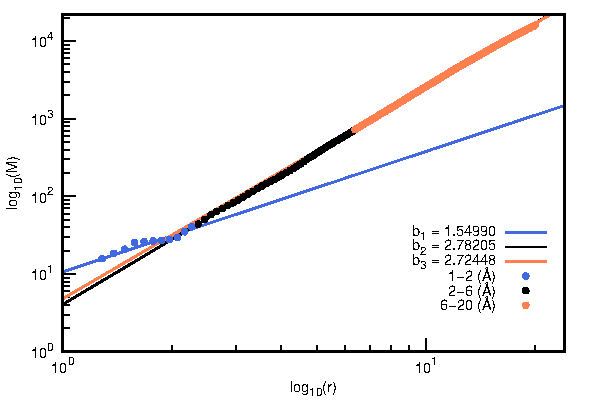
\includegraphics[width=\linewidth,page=1]{graphs/PDBs/1a52/1a52Eq.pdf}
		\caption{(3)}
	\end{subfigure}
	\hspace{0.2cm}
	\begin{subfigure}{0.49\textwidth} % M\'{a}s ancho para centrar
		\centering
		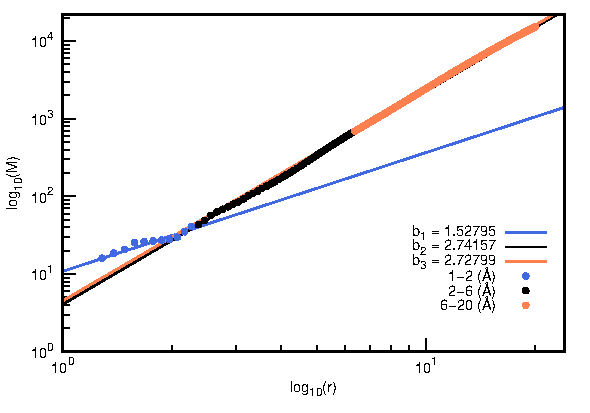
\includegraphics[width=\linewidth,page=1]{graphs/PDBs/1a52/1a521ns.pdf}
		\caption{(4)}
	\end{subfigure}
	\caption{Regresiones lineales de $\log_{10}r$ vs $\log_{10}M(r)$ correspondiente a cuatro etapas de procesamiento de la tercera prote\'{i}na con \textit{IdPDB:1a52} de la Tabla \ref{Tabla:ids9}: (1) Adici\'{o}n de \'{a}tomos de hidr\'{o}geno al sistema proteico; (2) al minimizar la energ\'{i´}a de la estructura molecular; (3) equilibrando el sistema bajo condiciones termodin\'{a}micas controladas; y (4) despu\'{e}s de una din\'{a}mica molecular de 1 ns.}
	\label{fig:1a52}
\end{figure}


\begin{figure}[H]
	\subsection*{IdPDB:1auk}
	\hspace{-0.3cm} 
	\begin{subfigure}{0.49\textwidth}
		\centering
		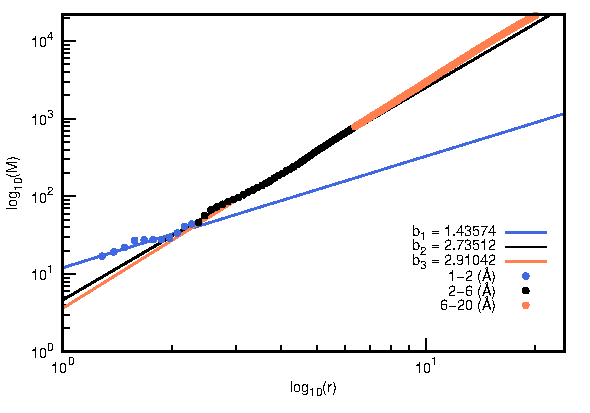
\includegraphics[width=\linewidth,page=1]{graphs/PDBs/1auk/1aukaddH.pdf}
		\caption{(1)}
	\end{subfigure}
	\hspace{0.2cm}
	\begin{subfigure}{0.49\textwidth}
		\centering
		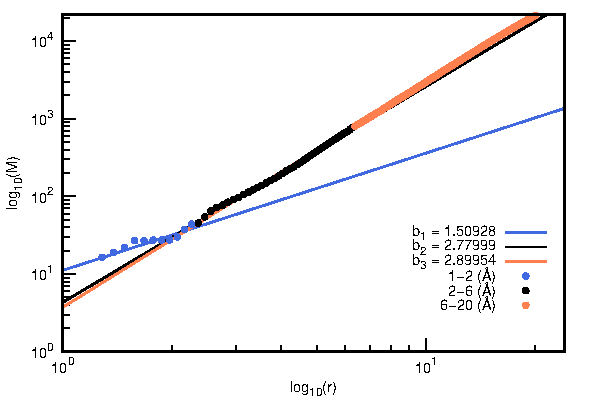
\includegraphics[width=\linewidth,page=1]{graphs/PDBs/1auk/1aukEm.pdf}
		\caption{(2)}
	\end{subfigure}
	
	\vspace{0cm} % Espacio entre filas
	
	\hspace{-0.3cm} 
	\begin{subfigure}{0.49\textwidth}
		\centering
		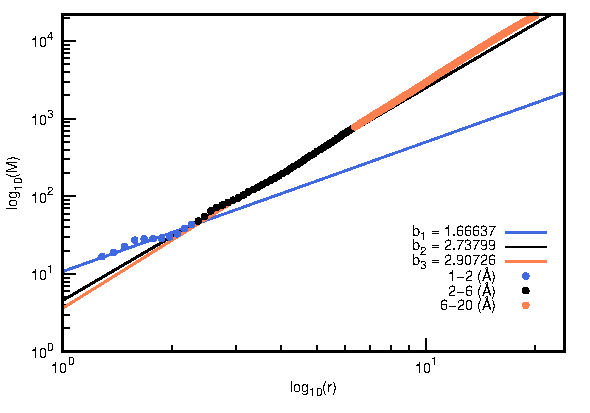
\includegraphics[width=\linewidth,page=1]{graphs/PDBs/1auk/1aukEq.pdf}
		\caption{(3)}
	\end{subfigure}
	\hspace{0.2cm}
	\begin{subfigure}{0.49\textwidth} % M\'{a}s ancho para centrar
		\centering
		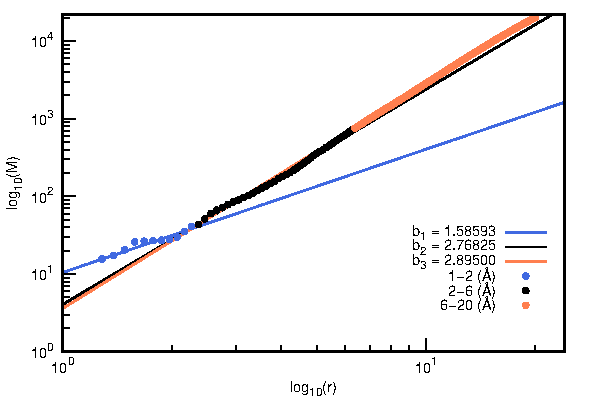
\includegraphics[width=\linewidth,page=1]{graphs/PDBs/1auk/1auk1ns.pdf}
		\caption{(4)}
	\end{subfigure}
	\caption{Regresiones lineales de $\log_{10}r$ vs $\log_{10}M(r)$ correspondiente a cuatro etapas de procesamiento de la sexta prote\'{i}na con \textit{IdPDB:1auk} de la Tabla \ref{Tabla:ids9}: (1) Adici\'{o}n de \'{a}tomos de hidr\'{o}geno al sistema proteico; (2) al minimizar la energ\'{i´}a de la estructura molecular; (3) equilibrando el sistema bajo condiciones termodin\'{a}micas controladas; y (4) despu\'{e}s de una din\'{a}mica molecular de 1 ns.}
	\label{fig:1auk}
\end{figure}

\begin{figure}[H]
	\subsection*{IdPDB:1b3e}
	
	\hspace{-0.3cm} 
	\begin{subfigure}{0.49\textwidth}
		\centering
		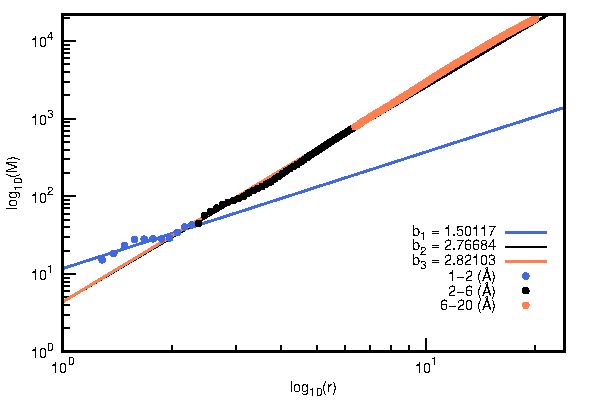
\includegraphics[width=\linewidth,page=1]{graphs/PDBs/1b3e/1b3eaddH.pdf}
		\caption{(1)}
	\end{subfigure}
	\hspace{0.2cm}
	\begin{subfigure}{0.49\textwidth}
		\centering
		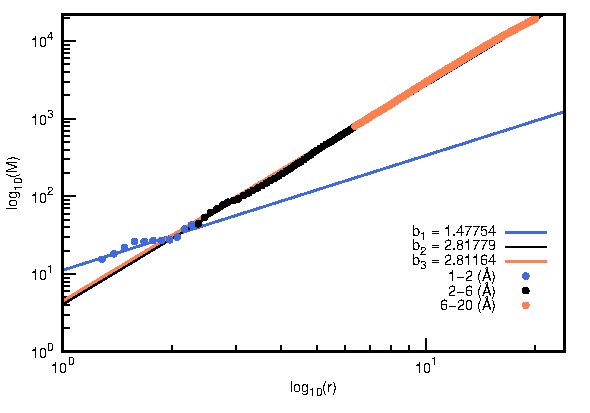
\includegraphics[width=\linewidth,page=1]{graphs/PDBs/1b3e/1b3eEm.pdf}
		\caption{(2)}
	\end{subfigure}
	
	\vspace{0cm} % Espacio entre filas
	
	\hspace{-0.3cm} 
	\begin{subfigure}{0.49\textwidth}
		\centering
		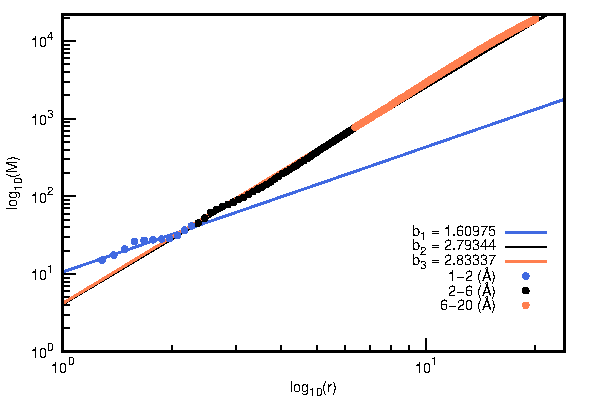
\includegraphics[width=\linewidth,page=1]{graphs/PDBs/1b3e/1b3eEq.pdf}
		\caption{(3)}
	\end{subfigure}
	\hspace{0.2cm}
	\begin{subfigure}{0.49\textwidth} % M\'{a}s ancho para centrar
		\centering
		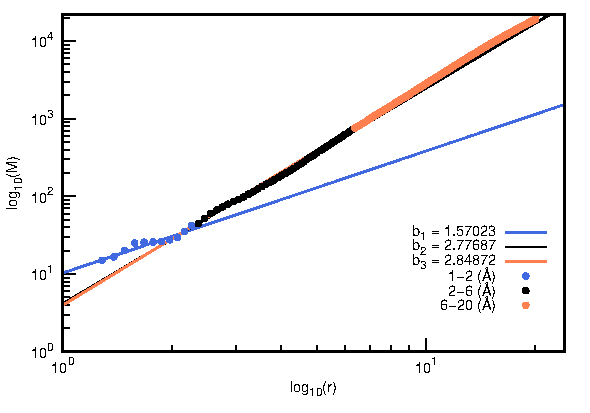
\includegraphics[width=\linewidth,page=1]{graphs/PDBs/1b3e/1b3e1ns.pdf}
		\caption{(4)}
	\end{subfigure}
	\caption{Regresiones lineales de $\log_{10}r$ vs $\log_{10}M(r)$ correspondiente a cuatro etapas de procesamiento de la s\'{e}ptima prote\'{i}na con \textit{IdPDB:1b3e} de la Tabla \ref{Tabla:ids9}: (1) Adici\'{o}n de \'{a}tomos de hidr\'{o}geno al sistema proteico; (2) al minimizar la energ\'{i´}a de la estructura molecular; (3) equilibrando el sistema bajo condiciones termodin\'{a}micas controladas; y (4) despu\'{e}s de una din\'{a}mica molecular de 1 ns.}
	\label{fig:1b3e}
\end{figure}


\begin{figure}[H]
	\subsection*{IdPDB:7khw}
	
	\hspace{-0.3cm} 
	\begin{subfigure}{0.49\textwidth}
		\centering
		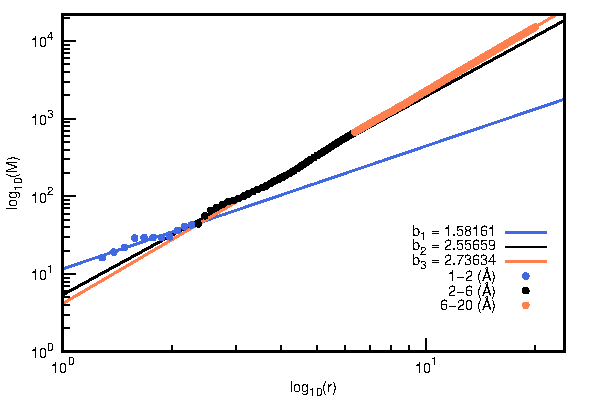
\includegraphics[width=\linewidth,page=1]{graphs/PDBs/7khw/7khwaddH.pdf}
		\caption{(1)}
	\end{subfigure}
	\hspace{0.2cm}
	\begin{subfigure}{0.49\textwidth}
		\centering
		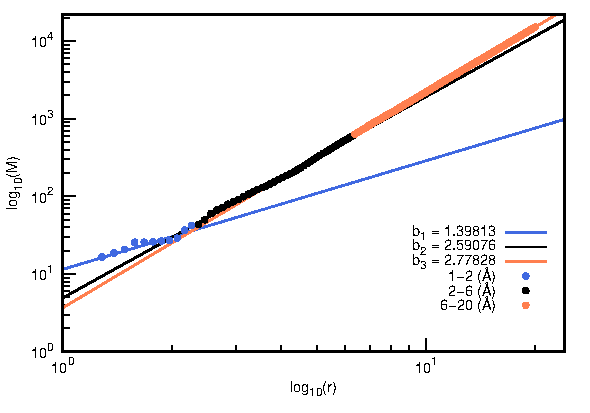
\includegraphics[width=\linewidth,page=1]{graphs/PDBs/7khw/7khwEm.pdf}
		\caption{(2)}
	\end{subfigure}
	
	\vspace{0cm} % Espacio entre filas
	
	\hspace{-0.3cm} 
	\begin{subfigure}{0.49\textwidth}
		\centering
		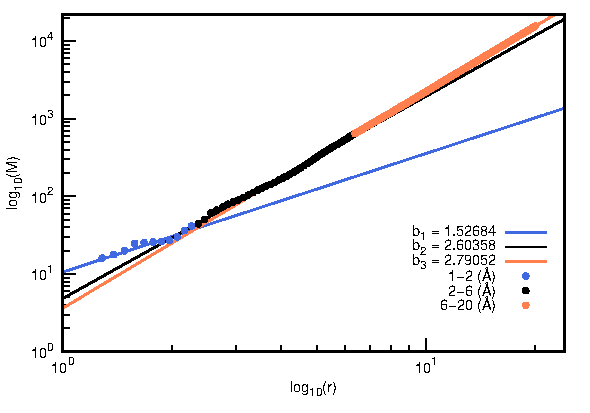
\includegraphics[width=\linewidth,page=1]{graphs/PDBs/7khw/7khwEq.pdf}
		\caption{(3)}
	\end{subfigure}
	\hspace{0.2cm}
	\begin{subfigure}{0.49\textwidth} % M\'{a}s ancho para centrar
		\centering
		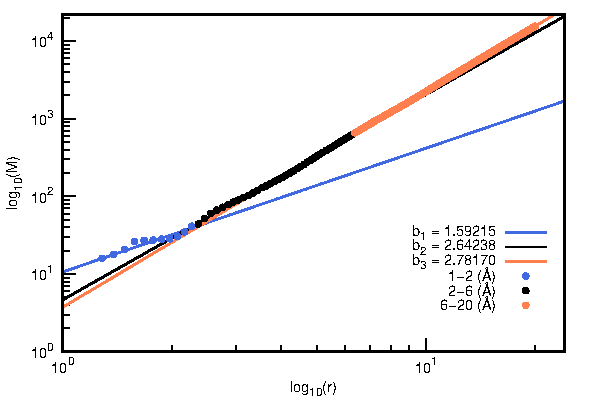
\includegraphics[width=\linewidth,page=1]{graphs/PDBs/7khw/7khw1ns.pdf}
		\caption{(4)}
	\end{subfigure}
	\caption{Regresiones lineales de $\log_{10}r$ vs $\log_{10}M(r)$ correspondiente a cuatro etapas de procesamiento de la novena prote\'{i}na con \textit{IdPDB:7khw} de la Tabla \ref{Tabla:ids9}: (1) Adici\'{o}n de \'{a}tomos de hidr\'{o}geno al sistema proteico; (2) al minimizar la energ\'{i´}a de la estructura molecular; (3) equilibrando el sistema bajo condiciones termodin\'{a}micas controladas; y (4) despu\'{e}s de una din\'{a}mica molecular de 1 ns.}
	\label{fig:7khw}
\end{figure}

\begin{figure}[H]
	\subsection*{IdPDB:11gs}
	
	\hspace{-0.3cm} 
	\begin{subfigure}{0.49\textwidth}
		\centering
		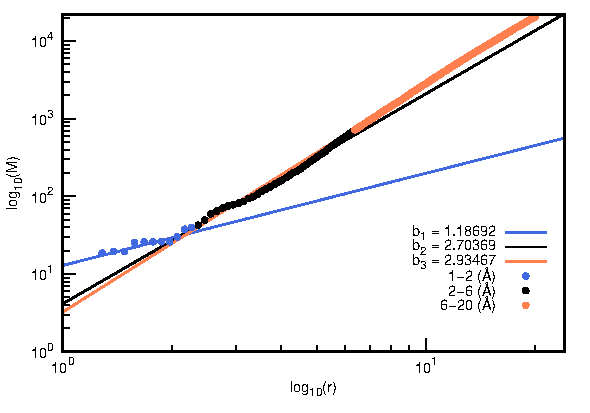
\includegraphics[width=\linewidth,page=1]{graphs/PDBs/11gs/11gsaddH.pdf}
		\caption{(1)}
	\end{subfigure}
	\hspace{0.2cm}
	\begin{subfigure}{0.49\textwidth}
		\centering
		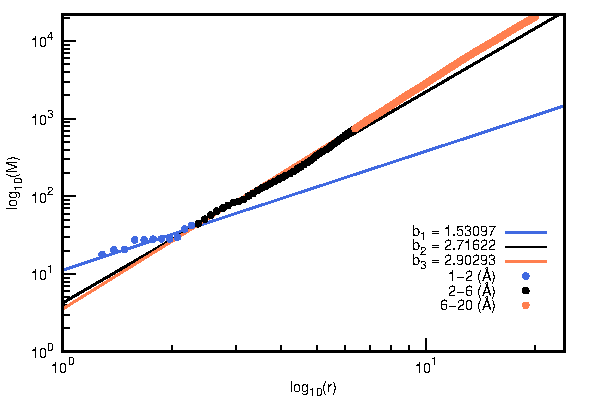
\includegraphics[width=\linewidth,page=1]{graphs/PDBs/11gs/11gsEm.pdf}
		\caption{(2)}
	\end{subfigure}
	
	\vspace{0cm} % Espacio entre filas
	
	\hspace{-0.3cm} 
	\begin{subfigure}{0.49\textwidth}
		\centering
		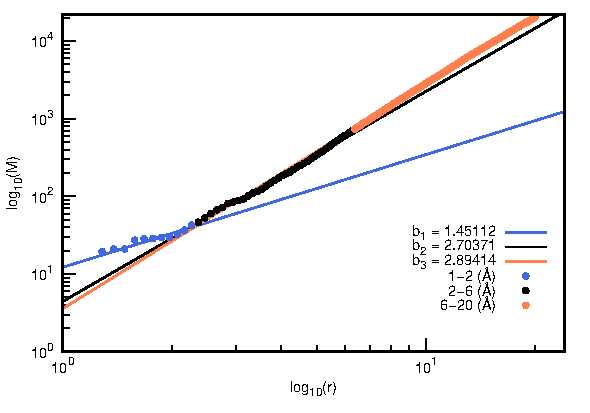
\includegraphics[width=\linewidth,page=1]{graphs/PDBs/11gs/11gsEq.pdf}
		\caption{(3)}
	\end{subfigure}
	\hspace{0.2cm}
	\begin{subfigure}{0.49\textwidth} % M\'{a}s ancho para centrar
		\centering
		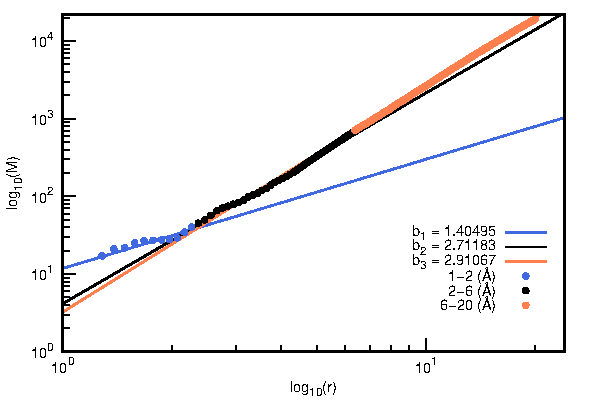
\includegraphics[width=\linewidth,page=1]{graphs/PDBs/11gs/11gs1ns.pdf}
		\caption{(4)}
	\end{subfigure}
	
	\caption{Regresiones lineales de $\log_{10}r$ vs $\log_{10}M(r)$ correspondiente a cuatro etapas de procesamiento de la octava prote\'{i}na con \textit{IdPDB:11gs} de la Tabla \ref{Tabla:ids9}: (1) Adici\'{o}n de \'{a}tomos de hidr\'{o}geno al sistema proteico; (2) al minimizar la energ\'{i´}a de la estructura molecular; (3) equilibrando el sistema bajo condiciones termodin\'{a}micas controladas; y (4) despu\'{e}s de una din\'{a}mica molecular de 1 ns.}
	\label{fig:11gs}
\end{figure}
´


